\section{VoLTE传输协议分析}
\label{chap:backinfo:rtp}

%VoLTE实在RTP协议的基础上实现的,RTP自身有一些特征
RTP是VoLTE使用的应用层协议,通过主动丢包的方式构建时间隐通道,需要对数据包进行准确辨别。
%在这里进行的分析,如何利用这些特征,构造时间隐通道
在RTP协议中,存在一些固定的字段及结构,利用这些字段,完成数据包身份的识别,以及时间隐通道保密性提升。

\subsection{RTP数据包结构}
\label{chap:backinfo:rtp:struct}

%RTP是怎样的标准,数据包等层次解析
RTP是以UDP作为传输层协议,不需要进行类似TCP的握手及挥手,也不会受到传输窗口的限制。因此,RTP在传输延迟及响应速度方面具有极大的优势,在实时音视频通话、互联网实时应用中得到广泛应用。\nupcite{6923336}根据数据包的结构组成,IP数据包的负载是封装的UDP数据包内容,UDP的负载是封装的RTP数据包内容。由于当前以太网的最大传输单元(MTU)通常设定为1500 Bytes,IPv6网络下IP包头长度通常为40 Bytes,UDP包头通常为8 Bytes,RTP包头通常为12 Bytes,RTP负载的数据通常不超过1440 Bytes。\nupcite{6269462}受限于网络参数,待发送的视频帧必须分包传输,增加了数据包数量。

\insertFigure{
	\begin{figure}
		\centering
        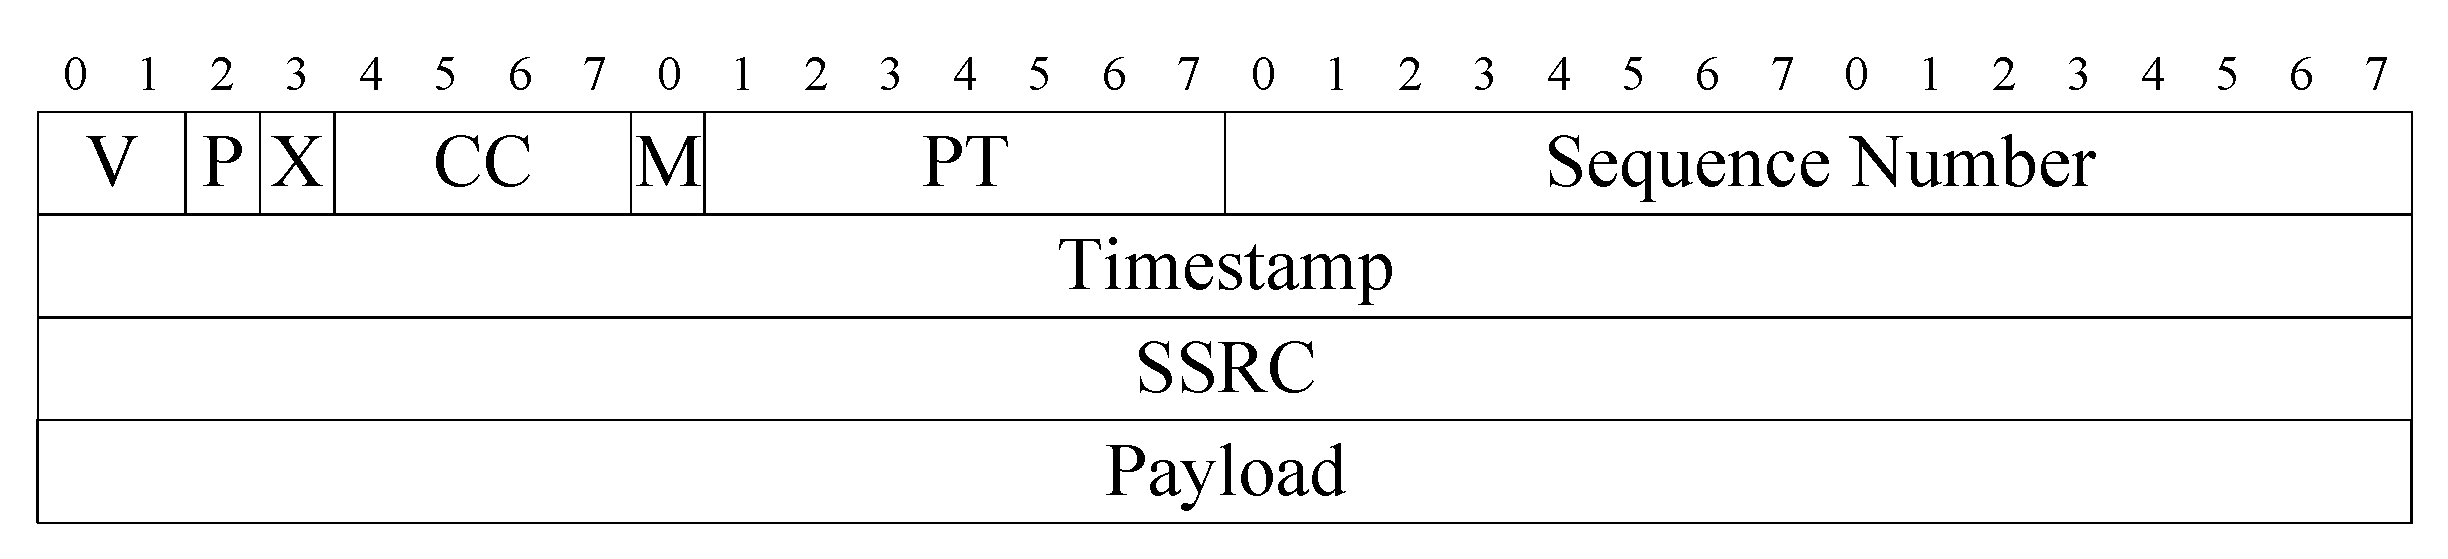
\includegraphics[width=0.9\textwidth]{chapters/chapter2/figures/rtp-header.pdf}
        \caption{RTP数据包头结构示意图}\label{fig:2:rtp-header}
	\end{figure}
}

%RTP头的组成
VoLTE中常见的RTP数据包头结构如图\nref{fig:2:rtp-header},在包头中存在固定的字段,如V(Version)表明RTP协议版本,M(Marker)指示负载分片的终止,PT(Payload Type)指明数据负载的类型。

\subsection{随机字段}
\label{chap:backinfo:rtp:random}

%RTP参数中,包含哪些随机生成的字段
RTP数据包头中,存在一些特殊的字段,其数据取值在标准中有隐含要求。

%SSRC、TimeStamp,生成的效果
图\nref{fig:2:rtp-header}中的Sequence Number字段,用于标识一次通话中的数据包顺序,按照间隔为1的规律递增。数据包序号的初始值应该随机生成,从而抵御已知明文攻击。

图\nref{fig:2:rtp-header}中的Timestamp字段,反映了采样时间的变化,便于接收方在网络抖动时,按照正确的时序进行数据处理。该字段的初始值也应该为随机值,在不同的传输流中,体现各自采样时间的变化。\nupcite{6156339}

图\nref{fig:2:rtp-header}中的SSRC(Synchronization Source identifier)字段,用于标记数据源。该字段取值必须随机生成,从而避免在一次RTP会话中出现相同的SSRC,如果发生了数据源的改变,该字段必须重新生成。SSRC字段的设计,实现了与特定数据流的对应,完成了流量标识。\nupcite{6222709}

%用于时间隐通道的秘钥及随机特征生成,保证保密性
时间隐通道作为隐蔽传输方法,传输的数据不应该被破解或截获。借助RTP中的这些随机字段和伪随机数生成算法,形成每次隐蔽传输的随机扰动,防范对隐通道的破坏。

\subsection{RTP丢包处理}
\label{chap:backinfo:rtp:dropout}

%RTP及应用中,对于丢包事件的处理
根据RTP数据包的层次,发生丢包后的处理结果,需要考虑各层次的相应行为。对于IP层来说,不会感知丢包事件,也不会出现重传行为;UDP本身没有重传及确认机制,无法保证数据包送达,也不存在重传行为;RTP重点在于实时性,而重传会破坏实时性效果,导致数据阻塞,因此只在RTCP数据包中进行反馈。\nupcite{6423613,5478577,6894614}

%丢包不重传,序号保证自增,是主动丢包方法的基础
RTP中数据包序号不重复、丢包后不重传,是基于主动丢包的时间隐通道的构造基础。对于隐通道发送方来说,在发送方丢弃的数据包,接收方一定可以感知到。数据包序号具有同步时钟的效果,时间隐通道根据序号范围分别进行丢包,无需附加同步时钟,确保了接收数据总量的一致性。